\usepackage{xcolor}
\usepackage{afterpage}
\usepackage{pifont,mdframed}
\usepackage[bottom]{footmisc}

\makeatletter
\gdef\this@inputfilename{input.txt}
\gdef\this@outputfilename{output.txt}
\makeatother

\newcommand{\inputfile}{\texttt{input.txt}}
\newcommand{\outputfile}{\texttt{output.txt}}

\newenvironment{warning}
  {\par\begin{mdframed}[linewidth=2pt,linecolor=gray]%
    \begin{list}{}{\leftmargin=1cm
                   \labelwidth=\leftmargin}\item[\Large\ding{43}]}
  {\end{list}\end{mdframed}\par}

La quarantaduesima edizione del campionato annuale delle formiche robot sta per cominciare, e quest'anno è compito di Giorgio decidere la prova che i concorrenti dovranno affrontare.

Dato il pasticcio che hanno combinato gli organizzatori della scorsa edizione (chi potrebbe mai dimenticare l'\emph{Arena con il formichiere}?), Giorgio ha deciso di puntare su qualcosa di più semplice: allestirà una griglia a mo' di labirinto (la \emph{Labigriglia}) e premierà la formica che la percorrerà nel modo più efficiente.

Una labigriglia non è altro che una pavimentazione formata da $N \times M$ mattonelle quadrate. Ad esempio, una labigriglia valida con $N=4$ e $M=6$ è visibile nella seguente figura:

\begin{center}
  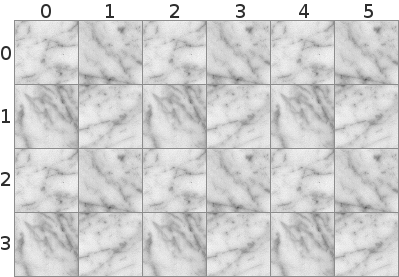
\includegraphics[width=0.8\textwidth]{floor.png}
\end{center}

L'obiettivo delle formiche robot è quello di partire dallo spigolo in alto a sinistra della mattonella $(0, 0)$ e arrivare allo spigolo in basso a destra della mattonella $(N-1, M-1)$ cercando però di non ``calpestare'' troppe mattonelle. La formica vincente è quella che calpesta il minor numero di mattonelle.

\begin{warning}
  Le formiche robot possono spostarsi da una mattonella all'altra tramite i lati o gli spigoli. Una formica può quindi spostarsi al massimo verso $8$ mattonelle (dallo stesso punto di partenza).
\end{warning}

Per rendere più interessante il gioco, Giorgio ha comprato un insetticida per formiche robot, e ha intenzione di spruzzarlo su alcune mattonelle. Una formica robot non può calpestare l'insetticida.

Se il giorno della gara Giorgio sarà di buon umore l'insetticida non verrà spruzzato. Se invece Giorgio sarà di cattivo umore, allora sceglierà una o più mattonelle e comincierà ad avvelenarle seguendo questa tecnica: all'inizio dirigerà il getto dell'insetticida verso il centro della mattonella, dopodiché continuerà a spruzzare muovendosi in una delle $4$ direzioni: verso l'alto, verso destra, verso il basso, verso sinistra.

Quindi, se Giorgio si dovesse sentire particolarmente malvagio, la ``traccia'' lasciata dall'insetticida potrà arrivare a formare un simbolo { \Large \color{magenta} \textbf{+} } nella mattonella. Ad esempio, nella seguente labigriglia ci sono due mattonelle posizionate in $(0, 2)$ e in $(2, 1)$ che sono state riempite di veleno!

\begin{center}
  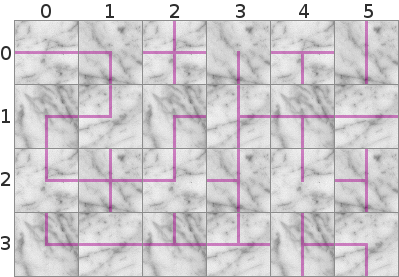
\includegraphics[width=0.8\textwidth]{floor-poison.png}
\end{center}

Per far capire ai partecipanti dove si trova il veleno e dove no, Giorgio definisce il ``fattore di velenosità'' per ciascuna mattonella. Questo fattore è inizialmente pari a $0$ per tutte le mattonelle. Durante l'applicazione dell'insetticida il fattore aumenta come segue:

\begin{itemize} %[noitemsep,nolistsep]
  \item Dal centro \emph{verso l'alto}: la velenosità della mattonella cresce di $1$;
  \item Dal centro \emph{verso destra}: la velenosità della mattonella cresce di $2$;
  \item Dal centro \emph{verso il basso}: la velenosità della mattonella cresce di $4$;
  \item Dal centro \emph{verso sinistra}: la velenosità della mattonella cresce di $8$.
\end{itemize}

\textbf{Nota:} questo valore non indica quindi \emph{quanto} è velenosa una mattonella, bensì \emph{dove} è velenosa.

\begin{warning}
  In pratica, il fattore di velenosità è un numero binario di $4$ bit. Se il bit meno significativo vale $1$, allora l'insetticida è stato spruzzato dal centro verso l'alto; se il secondo bit meno significativo vale $1$, allora l'insetticida è stato spruzzato dal centro verso destra; e così via.
\end{warning}

Aiuta Giorgio a organizzare la prossima edizione del campionato annuale delle formiche robot! Scrivi un programma che determini se una data labigriglia può essere risolta da una formica robot e, in tal caso, che calcoli anche il \emph{minimo numero di mattonelle} che essa dovrà calpestare per farlo.

\textbf{Nota:} se si passa più di una volta sulla stessa mattonella è necessario contarla di nuovo!

\Implementation
Dovrai sottoporre esattamente un file con estensione \texttt{.c}, \texttt{.cpp} o \texttt{.pas}.

\begin{warning}
Tra gli allegati a questo task troverai un template (\texttt{labigriglia.c}, \texttt{labigriglia.cpp}, \texttt{labigriglia.pas}) con un esempio di implementazione da completare.
\end{warning}

Se sceglierai di utilizzare il template, dovrai implementare la seguente funzione:
\begin{center}\begin{tabularx}{\textwidth}{|c|X|}
\hline
C/C++  & \verb|int cammina(int N, int M, int griglia[][MAXN]);|\\
\hline
Pascal & \begin{tabular}[x]{@{}@{}}\verb|type matrix = array of array of longint;|\\ \verb|function cammina(N, M: longint; var griglia: matrix): longint;|\end{tabular}\\
\hline
\end{tabularx}\end{center}
In cui:
\begin{itemize}[nolistsep]
  \item Gli interi $N$ e $M$ rappresentano rispettivamente il numero di righe e di colonne della labigriglia.
  \item La matrice \texttt{griglia}, indicizzata da $0$ a $N-1$ per le rige e da $0$ a $M-1$ per le colonne, descrive la labigriglia. In particolare \texttt{griglia[i][j]} è il fattore di velenosità della mattonella $(i, j)$.
  \item La funzione dovrà restituire il numero minimo di mattonelle che una formica robot deve calpestare per risolvere la labigriglia, oppure l'intero $-1$ se non fosse possibile risolverla.
\end{itemize}

\InputFile
Il file \inputfile{} è composto da $N+1$ righe. La prima riga contiene gli interi $N$ e $M$ separati da spazio. Le successive $N$ righe contengono ciascuna $M$ interi, e descrivono la matrice \texttt{griglia}.

\OutputFile
Il file \outputfile{} è composto da un'unica riga contenente l'intero $-1$ qualora non esistesse una soluzione, oppure un intero positivo: la risposta al problema.

% Assunzioni
\Constraints
\begin{itemize}[nolistsep, itemsep=2mm]
	\item $1 \le N, M \le 1000$.
	\item $0 \le$ \texttt{griglia[i][j]} $\le 15$ per ogni $i, j$.
\end{itemize}

\Scoring
Il tuo programma verrà testato su diversi test case raggruppati in subtask.
Per ottenere il punteggio relativo ad un subtask, è necessario risolvere
correttamente tutti i test relativi ad esso.

\begin{itemize}[nolistsep,itemsep=2mm]
  \item \textbf{\makebox[2cm][l]{Subtask 1} [10 punti]}: Casi d'esempio.
  \item \textbf{\makebox[2cm][l]{Subtask 2} [10 punti]}: \texttt{griglia[i][j]} $=0$ per ogni $i, j$. Niente veleno!
  \item \textbf{\makebox[2cm][l]{Subtask 3} [35 punti]}: $\min(N, M) = 1$. Diciamo che è più un \emph{labicorridoio}.
  \item \textbf{\makebox[2cm][l]{Subtask 4} [20 punti]}: $N, M \le 10$.
  \item \textbf{\makebox[2cm][l]{Subtask 5} [25 punti]}: Nessuna limitazione specifica.
\end{itemize}

% Esempi


\Examples
\begin{example}
\exmpfile{labigriglia.input0.txt}{labigriglia.output0.txt}%
\exmpfile{labigriglia.input1.txt}{labigriglia.output1.txt}%
\end{example}


\Explanation
Il \textbf{primo caso di esempio} corrisponde alla seconda figura presente nel testo. Un percorso che passa per $14$ mattonelle nella labigriglia in questione è il seguente:

\begin{center}
  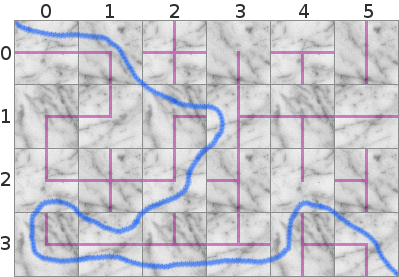
\includegraphics[width=0.8\textwidth]{floor-poison-path.png}
\end{center}
